\documentclass[conference]{IEEEtran}
\IEEEoverridecommandlockouts
% The preceding line is only needed to identify funding in the first footnote. If that is unneeded, please comment it out.
\usepackage{cite}
\usepackage{booktabs} % For formal tables
\usepackage{amsmath,amssymb,amsfonts}
\usepackage{algorithmic}
\usepackage{graphicx}
\usepackage{subcaption}
\usepackage{textcomp}
\usepackage{fancyhdr}
\usepackage{helvet}
\usepackage{xcolor}
\def\BibTeX{{\rm B\kern-.05em{\sc i\kern-.025em b}\kern-.08em
    T\kern-.1667em\lower.7ex\hbox{E}\kern-.125emX}}
\begin{document}

\title{Toon2real: A Technique for Cartoon to Photorealistic Image Synthesis\\
%{\footnotesize \textsuperscript{*}Note: Sub-titles are not captured in Xplore and
%should not be used}
}

\author{
\IEEEauthorblockN{K M Arefeen Sultan\IEEEauthorrefmark{1},
Labiba Kanij Rupty\IEEEauthorrefmark{2},
Mohammad Imrul Jubair\IEEEauthorrefmark{3},\\
Sayed Hossain Khan\IEEEauthorrefmark{4},
MD. Nahidul Islam\IEEEauthorrefmark{5}
}
\IEEEauthorblockA{
Department of Computer Science and Engineering,\\
Ahsanullah University of Science and Technology
Dhaka, Bangladesh\\
\{\IEEEauthorrefmark{1}krsultan069,
\IEEEauthorrefmark{2}labknr98,
\IEEEauthorrefmark{4}sayedhossainkhan36,
\IEEEauthorrefmark{5}nahidul19967\}@gmail.com,
\IEEEauthorrefmark{3}mohammadimrul.jubair@ucalgary.ca
}
}

\maketitle

\begin{abstract}
%*CRITICAL: Do Not Use Symbols, Special Characters, Footnotes, 
%or Math in Paper Title or Abstract.
In terms of Image-to-image translation, Generative Adversarial Networks (GANs) has achieved great success even when it is used in the unsupervised dataset. In this work, we aim to translate cartoon images to photorealistic images using GAN.
We apply several state-of-the-art models to perform this task; however, they fail to perform good quality translations.
We observe that shallow difference between these two domains causes this issue. Based on this idea, we propose a method based on CycleGAN model for image translation from cartoon domain to photorealistic domain. To make our model efficient, we implemented Spectral Normalization which added stability in our model. We demonstrate our experimental results and show that our proposed model has achieved the \textit{lowest Fr\'echet Inception Distance score} and better results compared to other state-of-the-art techniques, such as UNIT and SingleGAN.
\end{abstract}

\begin{IEEEkeywords}
GANs, Image-to-image-translation, Cartoon-to-real,
\end{IEEEkeywords}

\section{Introduction}
Cartoons occupy a huge part in our entertainment sector.
Film industries, in recent days, are remaking movies from the popular past cartoons and presenting them for current generation. Such an example is --
%In recent history, we have seen various movies
%such as 
the upcoming \textit{The Lion King (2019)} from \textit{The Lion king (1994)}. %\cite{lion_king_1}.
%where the cartoon domain is translated into the photorealistic domain. 
Therefore, we realize the necessity of recreating realistic images from the cartoons which can contribute to photorealistic rendering in computer graphics as well as in film industries. 
%Wouldn't it be amazing if the anime, cartoons we watch could be turned into real movies?
In this paper, we propose an approach which converts images from cartoons into their corresponding photorealistic images. From Figure~\ref{fig:intro}, we can see an outcome of our work where the cartoon scene is translated into a photorealistic one.

Image-to-image translation using Generative Adversarial Network (GAN)\cite{DBLP:conf/nips/GoodfellowPMXWOCB14} has been one of the most desiring fields of deep learning research lately. In a GAN architecure, a discriminator network tries to measure the probability of whether an image has come from an authentic data source or from a fake generated source of the generator. On the other hand, the generator tries to maximize the probability of the discriminator's making mistake and while doing that, it learns to generate more accurate data as much as close to real data. 
Tremendous success of GANs \cite{DBLP:conf/nips/GoodfellowPMXWOCB14}, led other researchers to work on unsupervised settings of datasets, such as \cite{DBLP:conf/iccv/ZhuPIE17}, \cite{DBLP:conf/icml/KimCKLK17}. Although these models have succeeded to translate one domain of image to another in general, there hasn't been any specific research for generating images of the photorealistic domain from cartoon domain.
This is an extremely hard task; the reason is the domain gap between these two distributions is too shallow.

\begin{figure}[!htb]
    \centering
    \begin{subfigure}[b]{0.2\textwidth}
        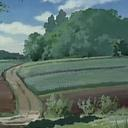
\includegraphics[scale=0.75]{Intro_pic/268.jpg}
        \caption{Cartoon scene}
        \label{subfig: intro1}
    \end{subfigure}
    \begin{subfigure}[b]{0.2\textwidth}
        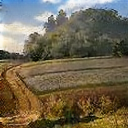
\includegraphics[scale=0.75]{Intro_pic/268_fake_B.png}
        \caption{Our result}
        \label{subfig:intro2}
    \end{subfigure}
    \caption{An example of cartoon to real world translation. (a) \textit{Input image}: which is from the animated film "My Neighbour Totoro". (b) \textit{Our result}: transforming the cartoon image (a) to real world image.}
    \label{fig:intro}
\end{figure}

As a result, the discriminator can be easily erroneous to determine the generated data as real ones.
This is the reason why most state-of-the-art models tend to fail in case of generating cartoon to real images. We illustrate in our result section that several models intent to keep the original content of cartoon domain while generating photo-realistic images.

To satisfy our objective on this task, we have taken an approach built on CycleGAN\cite{DBLP:conf/iccv/ZhuPIE17}. We implemented spectral normalization technique\cite{DBLP:journals/corr/abs-1802-05957} which helps our model to converge faster. Our approach also keeps the content of photo-realistic domain. In addition to these, we also created our own dataset for our model.
We show that our method has the {lowest FID score than the other baseline models and also, it tends to show more stabilization in training than the others}.

\section{Related Works}
In this section, we review on different relevant variations of GAN and several past works on image-to-image translations.

GANs have achieved great results in various image generation tasks, which are image super-resolution\cite{DBLP:journals/corr/JohnsonAL16}, image-to-image translation\cite{DBLP:conf/iccv/ZhuPIE17,DBLP:journals/corr/abs-1810-04991,DBLP:journals/corr/LiuBK17}, text-to-image synthesis\cite{DBLP:journals/corr/ZhangXLZHWM16,DBLP:journals/corr/ReedAYLSL16} etc. For stabilizing and improving the training of GAN, several works were proposed such as adding weight normalization and regularization techniques \cite{DBLP:journals/corr/GulrajaniAADC17, DBLP:journals/corr/abs-1802-05957}, designing new generative architectures\cite{DBLP:journals/corr/RadfordMC15, karras2017progressive} to improve visual results and modifying learning objectives \cite{Arjovsky2017WassersteinG,metz2016unrolled}. \textit{Miyato et al.}\cite{DBLP:journals/corr/abs-1802-05957} first proposed spectral normalization technique which constrains the Lipschitz constant of the discriminator network by limiting the spectral norm of each layer. 

% \parindent 5ex \textbf{Image-to-image translation.}
Recently, GAN\cite{DBLP:conf/nips/GoodfellowPMXWOCB14} based approach has given tremendous results in image-to-image translation tasks. \textit{Zhu et al.}\cite{DBLP:conf/iccv/ZhuPIE17} proposed a cycle consistency loss to reduce the infinite mappings of input images to any distribution in the target domain. \textit{Adversarial loss} alone can't solve the random permutation mappings of target distribution, rather it helps the input image to be translated into target domain. Similar to CycleGAN, \textit{Kim et al.} \cite{DBLP:conf/icml/KimCKLK17} proposed a method for preserving the key attributes between the input and the transformed image, while maintaining a cycle consistency criterion. Similarly,
%to cycle consistency, 
\textit{Yi et al.} \cite{yi2017dualgan} proposed dual-GAN mechanism based on dual learning from natural language translation\cite{he2016dual}.
In UNIT\cite{DBLP:journals/corr/LiuBK17} framework, \textit{Liu et al.} proposed a shared-latent space assumption, which denotes that the pair of corresponding images in different domains can be mapped to a same latent representation in a shared-latent space. \textit{Liu et al.} used the combination of generative adversarial network(GAN), based on CoGAN\cite{liu2016coupled} and variational autoencoders(VAEs)\cite{kingma2013auto,larsen2015autoencoding,rezende2014stochastic} .
Similarly to CycleGAN\cite{DBLP:conf/iccv/ZhuPIE17}, in SingleGAN\cite{DBLP:journals/corr/abs-1810-04991} framework, the authors used \textit{cycle consistency loss} \cite{DBLP:conf/iccv/ZhuPIE17}, where one generator is used instead of using two generators\cite{DBLP:conf/iccv/ZhuPIE17}.
In our previous work, CycleGAN based model was implemented to transform cartoon images into photo-realistic domain\cite{DBLP:journals/corr/abs-1811-11796}. While all these methods achieve compelling results, they take too much time for training. The reason behind it is that these models are not stabilized during training. Even after the training is finished, the models produce blurry or less vibrant results. In the next section we discuss on the approach we took to solve these fundamental issues and to obtain better outcomes.

\section{Formulation}

Our main objective is to transform \textit{cartoon} images to \textit{photo-realistic} images by learning the mapping of a \textit{cartoon} domain $C$ to the \textit{photo-realistic} domain $R$. To satisfy this objective, we adopted \textit{generative adversarial network}\cite{DBLP:conf/nips/GoodfellowPMXWOCB14} to train our models where, as mentioned earlier, $two$ networks will simultaneously learn the probability distribution of the domains, $C$ and $R$ to defeat each other respectively. In our case, the first network is a generator, $G_r: C\rightarrow R$ which learns the mapping between the distribution of domain $C$ and $R$ and will generate fake images $r_{fake}$, matched to domain $R$ using the mapping, whereas the second network,  Discriminator $D_r$ will learn the probability distribution of domain $R$ and try to differentiate between the generated images, $r_{fake}$ and the images $r$ from domain $R$. Our overall process is discussed below including our dataset preparation.

\parindent 5ex \textbf{Dataset Collection:} Due to the lack of paired data between {cartoon} domain and {photo-realistic} domain, we took an approach to collect unpaired dataset for both domains. We collected around $3.5K$ images from various \textit{cartoon} movies and scraped $6.2K$ images from \textit{Flickr} which were tagged as several categories like---\textit{scenery, sunrise, sunset, sea, sky, beach} etc. 
%However, to maintain a balance between the $two$ domains, we eliminated the first and last few minutes from the \textit{cartoon} movies while scraping. Also, we eliminated all the identical, shaky and completely dark images from the dataset.

\parindent 5ex \textbf{Adversarial Loss:} Although in
%the original paper
\cite{DBLP:conf/nips/GoodfellowPMXWOCB14}, a binary cross-entropy based Adversarial Loss function was proposed, we use a \textit{Least Squares Loss(LSGAN)} function for our training. According to \textit{Mao et. al} \cite{DBLP:conf/iccv/MaoLXLWS17}, we have explored that \textit{LSGAN} performs better in the case of vanishing gradient problem and thus shows more stability during training and produces much more higher quality images in the case of \textit{Image-to-image Translation}. So, our adversarial loss stands as follows - 

\begin{equation}
For\, Generator\, G_r,\, \mathcal{L}_{G_r}\, =\, \frac{1}{m}\sum^m_{i=1}(1-D_r(G_r(c)))^2
\end{equation}

However, due to the deep similarities between cartoon and photo-realistic images, we observed that, using only a single generator fails to map the differences between these $two$ domains. To resolve this issue, we use $two$ additional networks in our model, where a generator, $G_c$ tries to generate images of \textit{Cartoon} domain and a discriminator, $D_c$ tries to discriminate the generated image from \textit{cartoon} domain. The additional networks also perform according to the previously mentioned loss function.\\ %Unfinished.."real cartoon domain"?
\begin{figure}[!htb]
    \centering
    \begin{subfigure}[b]{0.2\textwidth}
        \centering
        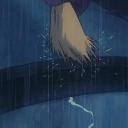
\includegraphics[scale=0.7]{Intro_pic/kds_real.png}
        \caption{Input from Cartoon Domain}
        \label{subfig: rc_1}
    \end{subfigure}
    \hspace{0.1in}
    \begin{subfigure}[b]{0.2\textwidth}
        \centering
        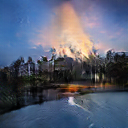
\includegraphics[scale=0.7]{Intro_pic/kds_fake.png}
        \caption{Output without Reconstruction Loss}
        \label{subfig:rc_2}
    \end{subfigure}
    \caption{(a) A scene taken from "Kiki's Delivery Service". (b) Translated output of image (a), without reconstruction loss, where the model generates an incomprehensible structure.}
    \label{fig:rc_loss}
\end{figure}

\parindent 5ex \textbf{Reconstruction Loss:} Adding an additional generator solves the issue of mapping differences; however it still lacks in content preservation. We noticed from our training that, while training with only adversarial loss, the model tends to produce images which fail to match with the input data. It happens because of multiple mappings of the target domain. For example, in Figure~\ref{fig:rc_loss} the generator(without reconstruction loss) generated an image, with some unstructured pixels in the middle which consists of multiple mappings of the target domain.

However, using an additional loss function, by using the technique of forward and backward loss\cite{DBLP:conf/icml/KimCKLK17, DBLP:conf/iccv/ZhuPIE17}, we've solved this content issue and have kept the similarities in the domain translation. The motive of this function is that, an image generated from an input can be reconstructed back to the input again such that $x = F(G(x))$, where $F$ and $G$ are generators and thus, it is able to map an image of target domain which is as close as possible to the image of input domain. In our paper, we call it \textit{Reconstruction Loss}. The equation is as follows - 
\begin{equation}
Forward\, Consistency\, Loss,\mathcal{L}_{f\_cyc} = \frac{1}{m} \sum^m_{i=1}(F_r(G_r(c)) - c)    
\end{equation}
\begin{equation}
Backward\, Consistency\, Loss,\mathcal{L}_{b\_cyc} = \frac{1}{m} \sum^m_{i=1}(G_r(G_c(r)) - r) 
\end{equation}

\parindent 5ex \textbf{Training Stabilization:}
Training GAN with efficiency is a hard nut to crack. Prior to previous works, it is known that, discriminator tends to make the training slower and show more inconsistency during training. We used \textit{Spectral Normalization} technique, which was first proposed by \textit{Miyato et al.}\cite{DBLP:journals/corr/abs-1802-05957}, to stabilize our training. Benefit of spectral normalization is that it doesn't need extra hyper-parameter tuning. Also, the computational cost is relatively small compared to other weight normalization techniques. \textit{Miyato et al.}\cite{DBLP:journals/corr/abs-1802-05957} found better or same results with image generation tasks by utilizing this normalization technique. We can see from Figure~\ref{fig:fid_graph}  that, using this technique stabilized the training, where Figure~\ref{subfig:fid_spectral} is ours, which shows a much smoother curve of FID scores than Figure~\ref{subfig:fid_cycle}, which is the FID score-graph of CycleGAN\cite{DBLP:conf/iccv/ZhuPIE17}. Also, we can see that ours achieved the least FID score within 145 epoch, whereas CycleGAN\cite{DBLP:conf/iccv/ZhuPIE17} takes more epochs for that.


\parindent 5ex \textbf{PatchGAN:}
As discriminators, we used PatchGAN which was first proposed in \textit{Isola et al.} \cite{DBLP:conf/cvpr/2017}. The intuition of using this discriminator is that it works best for extracting the high-frequency details of the distribution. Another beneficial feature is, due to working on $N\times N$ patches, it takes fewer parameters and thus decreases the computation cost.

\section{Implementations \& Analysis} \label{sec:imp}
In this section, we discuss the implementation of our approach followed by illustrating its results.

\parindent 5ex \textbf{Network structure:}
For generative networks we implemented the architecture from \textit{Johnson et al.} \cite{DBLP:journals/corr/JohnsonAL16} who achieved amazing results for neural style transfer and super-resolution. The network includes two stride-2 convolutions, $6$ residual blocks\cite{DBLP:journals/corr/HeZRS15}, and two fractional strided convolutions with stride $1/2$. We used instance normalization technique. For the discriminator network, we used $70\times70$ PatchGANs\cite{DBLP:conf/cvpr/2017}.
 
% table of FID scores
\begin{table}[!htb]
\centering
\caption{Fid scores of ours, UNIT and SingleGAN models.}
\large\addtolength{\tabcolsep}{0pt}
\begin{tabular}{ |c|c|c|c| } 
 \hline
 Models & Our Work & UNIT & SingleGAN \\ 
 \hline
 FID & \textbf{48.4225} & 55.9214 & 54.0130 \\
 \hline  
\end{tabular}

\label{fid_table}
\end{table}
\parindent 5ex \textbf{Evaluation metric:}
We chose the Fr\'echet Inception Distance (FID) \cite{DBLP:journals/corr/HeuselRUNKH17} for quantitative evaluation. As FID score measures the difference between the generated dataset and the target dataset, it has shown more consistency with human evaluation. it calculates the Wasserstein-2 distance between the translated image and the real world images from an intermediate layer of an Inception-v3 network. Lower the FID score, the closer the distance between translated image and real domain images. As our task is image-to-image translation where we want our output to have the content of input cartoon images and the style of real-world images, we calculated a weighted average between them, where we used $80\%$ weight for target data and $20\%$ weight for input data. From Table~\ref{fid_table} we can see that our work has shown the least FID score compared to other state of the art models.

\begin{figure}[!htb]
\begin{center}
    \begin{subfigure}[b]{0.35\textwidth}
        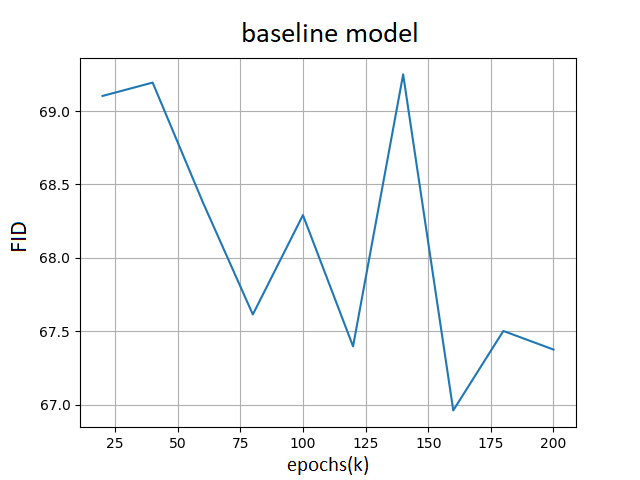
\includegraphics[scale=0.38]{graphs/(Orig)fid_82.png}
        \caption{CycleGAN model}
        \label{subfig:fid_cycle}
    \end{subfigure}
    \begin{subfigure}[b]{0.35\textwidth}
        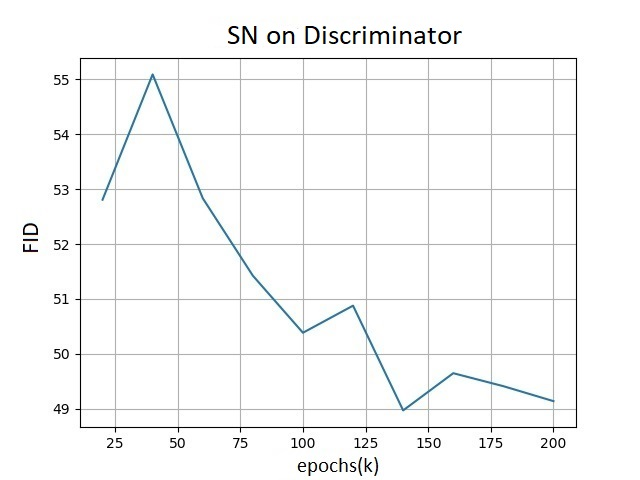
\includegraphics[scale=0.38]{graphs/Spectral_FID.jpg}
        \caption{Ours}
        \label{subfig:fid_spectral}
    \end{subfigure}
    \caption{Here, FID scores for CycleGAN (a) and for our method (b) are shown from $20$ epochs up to $200$ epochs.}
    \label{fig:fid_graph}
\end{center}
\end{figure}
%zoomed-image
\begin{figure*}[!htb]
\begin{center}
     \begin{subfigure}[normal]{0.2\textwidth}
         \label{Fig2 input}
         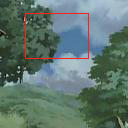
\includegraphics[scale = 0.7]{zooming_picture/in_x.jpg}
     \end{subfigure}
     \hspace{0.0001mm}
     \begin{subfigure}[normal]{0.2\textwidth}
         \label{subfig:B}
         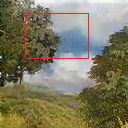
\includegraphics[scale = 0.7]{zooming_picture/our_x.jpg}
     \end{subfigure}
     \hspace{0.0001mm}
     \begin{subfigure}[normal]{0.2\textwidth}
         \label{subfig:C}
         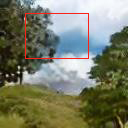
\includegraphics[scale = 0.7]{zooming_picture/unit_x.jpg}
     \end{subfigure}
     \hspace{0.0001mm}
     \begin{subfigure}[normal]{0.2\textwidth}
         \label{subfig:D}
         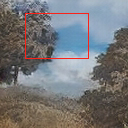
\includegraphics[scale = 0.7]{zooming_picture/sgan_x.jpg}
     \end{subfigure}
     \\
     \begin{subfigure}[normal]{0.2\textwidth}
         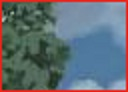
\includegraphics[scale = 0.7]{zooming_picture/in_y.jpg}
         \caption{Input}
     \end{subfigure}
     \hspace{0.0001mm}
     \begin{subfigure}[normal]{0.2\textwidth}
         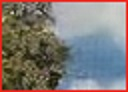
\includegraphics[scale = 0.7]{zooming_picture/our_y.jpg}
         \caption{Our work}
     \end{subfigure}
     \hspace{0.0001mm}
     \begin{subfigure}[normal]{0.2\textwidth}
         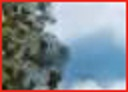
\includegraphics[scale = 0.7]{zooming_picture/unit_y.jpg}
         \caption{UNIT}
    \end{subfigure}
     \hspace{0.0001mm}
     \begin{subfigure}[normal]{0.2\textwidth}
         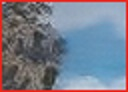
\includegraphics[scale = 0.7]{zooming_picture/sgan_y.jpg}
         \caption{SingleGAN}
     \end{subfigure}
     \caption{Detailed comparisons in terms of contrast and content preservation. (a) Input image of a cartoon scene (a portion is amplified inside red bounding box for better observation). (b) \textit{Result of our work}: shows more contrast on content, compared to other works. (c) \textit{Result of UNIT}\cite{DBLP:journals/corr/LiuBK17} which shows blurry content than (b). (d) \textit{Result of SingleGAN}: which doesn't provide real world colorization on tree leaves and grasses; the image became faded and less vibrant.} 
     \label{fig:compare}
\end{center}
\end{figure*}
%more results
\begin{figure*}[!htb]
\begin{center} %1st row
     \begin{subfigure}[normal]{0.2\textwidth}
         \label{subfig:A}
         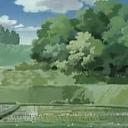
\includegraphics[scale = 0.7]{pic/in_2.jpg}
     \end{subfigure}
     ~
     \begin{subfigure}[normal]{0.2\textwidth}
         \label{subfig:B}
         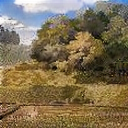
\includegraphics[scale = 0.7]{pic/our_2.png}
     \end{subfigure}
     ~
     \begin{subfigure}[normal]{0.2\textwidth}
         \label{subfig:D}
         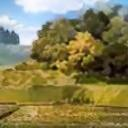
\includegraphics[scale = 0.7]{pic/unit_2.jpg}
     \end{subfigure}
     ~
     \begin{subfigure}[normal]{0.2\textwidth}
         \label{subfig:E}
         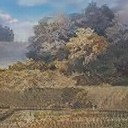
\includegraphics[scale = 0.94]{pic/sgan_2.jpg}
     \end{subfigure}
     \\%2nd row
     \begin{subfigure}[normal]{0.2\textwidth}
         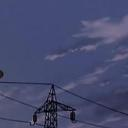
\includegraphics[scale = 0.7]{pic/96.jpg}
     \end{subfigure}
     ~
     \begin{subfigure}[normal]{0.2\textwidth}
         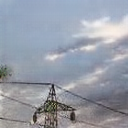
\includegraphics[scale = 0.7]{pic/cycle_spec96.png}
     \end{subfigure}
     ~
     \begin{subfigure}[normal]{0.2\textwidth}
         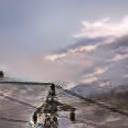
\includegraphics[scale = 0.7]{pic/outputUNIT96.jpg}
     \end{subfigure}
     ~
     \begin{subfigure}[normal]{0.2\textwidth}
         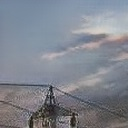
\includegraphics[scale = 0.93]{pic/singlegan96.jpg}
     \end{subfigure}
     \\%3rd row
     \begin{subfigure}[normal]{0.2\textwidth}
         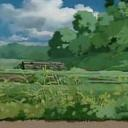
\includegraphics[scale = 0.7]{pic/in_3.jpg}
         \caption{Input}
     \end{subfigure}
     ~
     \begin{subfigure}[normal]{0.2\textwidth}
         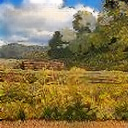
\includegraphics[scale = 0.7]{pic/our_3.png}
         \caption{Our work}
     \end{subfigure}
     ~
     \begin{subfigure}[normal]{0.2\textwidth}
         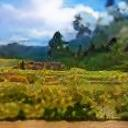
\includegraphics[scale = 0.7]{pic/unit_3.jpg}
         \caption{UNIT}
     \end{subfigure}
     ~
     \begin{subfigure}[normal]{0.2\textwidth}
         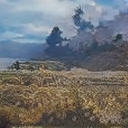
\includegraphics[scale = 0.7]{pic/sgan_3.jpg}
         \caption{SingleGAN}
     \end{subfigure}
     \caption{More qualitative results of our work compared to others. (a) Input images of cartoon scenes. (b) \textit{Results of our work}: the results are much more vibrant and can preserve the content of input image compared to other models. (c) \textit{Results of UNIT}\cite{DBLP:journals/corr/LiuBK17}: which sometimes fail to preserve the content of input image and makes image blurry or too much smooth. (d) \textit{Results of SingleGAN}\cite{DBLP:journals/corr/abs-1810-04991}: which makes the overall image less vibrant and sometimes fail to keep content preservation.}
     \label{fig:more results}
\end{center}
\end{figure*}
\parindent 5ex \textbf{Evaluation of stabilization technique:}
By utilizing spectral normalization technique on discriminator network shown in Figure \ref{subfig:fid_spectral}, we started to gain lower FID score from the very initial of training compared to baseline model, which is implemented based on CycleGAN\cite{DBLP:conf/iccv/ZhuPIE17} model. Spectral normalization is used on discriminator network on baseline model which is shown in \ref{subfig:fid_spectral}. From \ref{subfig:fid_spectral}, the quality of transforming images doesn't improve monotonically during training. For example, the FID score of our work starts to drop at the $37$th epoch. On the contrary, baseline model's FID score starts to rise after $125$th epoch and it crosses the initial FID scores, whereas in our work, the scores didn't rise like the baseline model did. From this, we can clarify that we achieved a more stabilized model and better scores. We can also clarify from Figure \ref{fig:fid_graph} that the stabilization technique also takes fewer training epochs to achieve better scores. %Unfinished writing..last line er aager line.


\parindent 5ex \textbf{Comparison with state of the art models:}
We compared our work with state of the art techniques, i.e UNIT \cite{DBLP:journals/corr/LiuBK17} and SingleGAN's base model\cite{DBLP:journals/corr/abs-1810-04991}. In Figure \ref{fig:compare}, we show a close-up view of an example, explaining that our work preserves much better vibrance and content preservation, where UNIT's\cite{DBLP:journals/corr/LiuBK17} output becomes blurred and SingleGAN\cite{DBLP:journals/corr/abs-1810-04991} makes unrealistic color on the content of output image.  %Unfinished about zoomed-image SingleGAN.
In Figure \ref{fig:more results}, we showed that our work achieved more color consistency and content preservation in cartoon to real world domain translation task. The UNIT\cite{DBLP:journals/corr/LiuBK17} framework fails to keep content preservation of input images where it makes the content blurry. SingleGAN\cite{DBLP:journals/corr/abs-1810-04991} results are overall less vibrant, it couldn't preserve the real world images colorization and sometimes the model fails to preserve the content of input image.

%limitation output
\begin{figure}[!htb]
    \centering
    \begin{subfigure}[b]{0.2\textwidth}
        \centering
        
\includegraphics[scale=0.7]{limitation/cat_real_A.png}
        \caption{Cartoon scene}
    \end{subfigure}
    \begin{subfigure}[b]{0.2\textwidth}
        \centering
        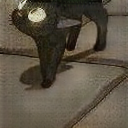
\includegraphics[scale=0.7]{limitation/cat_fake_B.png}
        \caption{Our result}
    \end{subfigure}
    \caption{
    %Similar to UNIT\cite{DBLP:journals/corr/LiuBK17} and other image-to-image translation models, 
    A failure case of our method. In the output image (b), the \textit{cat} remains cartoonish as in input (a) and is not translated into a realistic one.}
    \label{fig:limitation}
\end{figure}

\parindent 5ex \textbf{Limitations:} Despite achieving better FID score of all, it is still too high to be a perfect image translation score. In fact, we can see from Figure~\ref{fig:limitation} that, the output fails to achieve the
%geometric 
meaningful (semantically and geometrically)
structure of real-world objects---in this example a \textit{cat}.
This problem is also common in UNIT\cite{DBLP:journals/corr/LiuBK17} and other image-to-image translation models.
%In real world cats don't have big eyes like our result does. So our model fails to preserve semantic content of output domain.

\section{Conclusion}

In this paper, we showed a GAN based approach to translate images from cartoon domain to photo-realistic domain. We implemented our model based on CycleGAN\cite{DBLP:conf/iccv/ZhuPIE17}, where we used Reconstruction Loss for content preservation of input image and the PatchGAN for better texture extraction. By implementing spectral normalization technique on discriminator network, we showed that our model achieves better training stability and the lowest FID score of all the other models. Our future plan is to lessen our current limitations by investigating more geometry and content aware model to improve the texture so that the gap with the photorealistic domain decreases. In addition to FID score, we have plans to arrange human-involved and perceptual evaluation processes to asses the correctness of your outcomes.

\bibliographystyle{IEEEtran}
\bibliography{sample-bibliography}
\newpage
\onecolumn

\begin{flushleft}
\begin{center}
\Huge \textbf{AUTHORS' BACKGROUND}    
\end{center}


\normalsize
\begin{table*}[!htb] 
\renewcommand{\arraystretch}{3}
\normalsize\addtolength{\tabcolsep}{10pt}
\begin{tabular}{ |c|c|c|c| }

 \hline
Your Name & Position & Research Field & Personal Webpage \\ 
 \hline 
 K M Arefeen Sultan & Bachelor Student   & Computer Vision &  \\
 \hline
 Labiba Kanij Rupty &  Bachelor Student   &  Computer Vision  &  \\
 \hline
  Mohammad Imrul Jubair & Assistant Professor   & Computer Graphics, Computer Vision  &  https://imruljubair.github.io \\
 \hline
 Sayed Hossain Khan &  Bachelor Student   &  Computer Vision  &  \\
 \hline
 MD. Nahidul Islam &  Bachelor Student   & Computer Vision  &  \\
 \hline
\end{tabular}
\renewcommand{\arraystretch}{1}
\end{table*}

\end{flushleft}
\normalsize


\end{document}
